\documentclass[handout]{beamer}
\usetheme{default}

\usepackage{graphicx} % \includegraphics
\usepackage{mathrsfs} % \mathscr

% to print with notes
\setbeameroption{show notes}

% no decoration to notes
%\setbeamertemplate{note page}[plain]

% http://tex.stackexchange.com/questions/66995/modify-footer-of-slides
\makeatother
\setbeamertemplate{footline}
{
  \leavevmode
  \hbox{
  \begin{beamercolorbox}[wd=.4\paperwidth,ht=2.25ex,dp=1ex,center]{author in head/foot}
    \usebeamerfont{author in head/foot}\insertshortauthor
  \end{beamercolorbox}
  \begin{beamercolorbox}[wd=.6\paperwidth,ht=2.25ex,dp=1ex,center]{title in head/foot}
    \usebeamerfont{title in head/foot}\insertshorttitle\hspace*{3em}
    \insertframenumber{} / \inserttotalframenumber\hspace*{1ex}
  \end{beamercolorbox}}
  \vskip0pt
}
\makeatletter
\setbeamertemplate{navigation symbols}{}

\begin{document}

\title{Cluster algorithms for the Ising model}
\author{Roger Walt}

\begin{frame}
	\huge{Cluster algorithms for the Ising model}
	\vspace*{5pt}

	\Large{Monte Carlo methods which overcome the problem of critical slowing down close to second order phase transitions}
\end{frame}

\begin{frame}{Ising model - Why?}
\begin{columns}[c]
	\column{.5\textwidth}
	\begin{itemize}
		\item<1-> Phase transitions.
			\note[item]<1> {Phase transitions are important}
		\item<2-> One of the simplest statistical models that show a phase transition.
			\note[item]<2> {The Ising model is one of the simplest statistical models that shows a phase transition.}
		\item<3-> Magnetic systems, opinion models, binary mixtures
			\note[item]<3> {Ising model can be used to simulate magnetic systems (ferromagnetic and antiferromagnetic), opinion models and binary mixtures.}
	\end{itemize}
	\column{.5\textwidth}
	\pause[4]
	\begin{figure}[p]
		\centering
		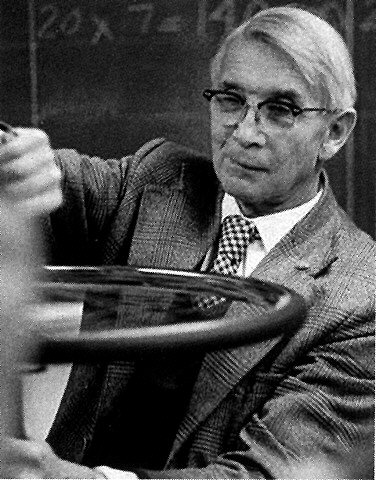
\includegraphics{img/ising.jpg}
		\caption{Ernst Ising (1900 - 1998)}
		\label{fig:awesome_image}
	\end{figure}
	\note<4> {Figure: Ernst Ising, lived from 1900 to 1998}
	\note[item]<4> {Ising model invented by Wilhelm Lenz (1888 - 1957) (the same as the Lenz in the Laplace-Runge-Lenz vector) in 1920, his student Ernst Ising solved it in the one-dimensional case 1924.}
	\note[item]<4> {Wolfgang Pauli (1900 - 1958), at whom the road outside is named after, was an assistant of Lenz.}
	\note[item]<4> {Also Otto Stern (1888 - 1969) from the Stern-Gerlach experiment was an assistant of Lenz.}
\end{columns}
\end{frame}

\begin{frame}{Ising model - Definition}
\begin{itemize}
\item<2-> Lattice with \(N\) sites
\item<3-> Discrete integer spins \( \sigma_i = \pm 1 \) on each lattice site
\item<4-> \[ \mathscr{H}(\sigma) = -J \sum\limits_{i, j} \sigma_i \sigma_j - \mu H \sum\limits_i \sigma_i \]
	\note[item]<5> {More favorable for the spins to be aligned!}
\item<5-> \( J \): interaction, \( H \): external field
	\note[item]<5> {\( J_{ij} \) in general case, \( J>0 \): ferromagnetic, \( J<0 \): antiferromagnetic}
\item<6-> \[ p(\sigma, T) = \frac{e^{-\beta \mathscr{H}(\sigma)}}{\mathscr{Z}(T)}, \ \ \ \ \beta=\frac{1}{k_B T}\]
	\note[item]<6> {Configuration probability given by boltzmann distribution, Z partition function, given as \[ \mathscr{Z}(T) = \sum_\sigma e^{-\beta \mathscr{H}(\sigma)},\ \ \beta = \frac{1}{k_B T} \]}
	\note[item]<6> {So we are looking at a canonical system with constant temperature T.}
\item<7-> \[ \left< M \right>|_T = \sum_\sigma M(\sigma)p(\sigma,T) \]
	\note[item]<7> {Measurement value of a function, e.g. magnetization, is given by the sum over all states of the measurement value at the configuration times the configuration probability.}
\end{itemize}
\end{frame}

\begin{frame}{Ising model - Monte Carlo}
\begin{itemize}
\item<2-> We can't compute all configurations.
	\note[item]<2> {Why not? \( \rightarrow 2^N = 2^{L^d} \) e.g. \( L = systemSize = 15 \) in 2 dimensions: \(2^{15^2} = 2^{225} = 5 \cdot 10^{67}\)}
	\note[item]<2> {We can't compute the exact expectation value of an observable. But that's what we're interested in.}
\item<3-> We don't want to sample equally distributed over energy.
	\note[item]<3> {Because the distribution of the average energy gets sharper with increasing size \(\left(\alpha \ \sqrt{L^d}\right)\).}
\end{itemize}
\end{frame}











\begin{frame}{A sample slide}

A displayed formula:

\[
  \int_{-\infty}^\infty e^{-x^2} \, dx = \sqrt{\pi}
\]

An itemized list:

\begin{itemize}
  \item itemized item 1
  \item itemized item 2
  \item itemized item 3
\end{itemize}

\begin{theorem}
  In a right triangle, the square of hypotenuse equals
  the sum of squares of two other sides.
\end{theorem}

\end{frame}

\end{document}
